% \IUref{IUAdmPS}{Administrar Planta de Selección}
% \IUref{IUModPS}{Modificar Planta de Selección}
% \IUref{IUEliPS}{Eliminar Planta de Selección}



% Copie este bloque por cada caso de uso:
%-------------------------------------- COMIENZA descripción del caso de uso.

%\begin{UseCase}[archivo de imágen]{UCX}{Nombre del Caso de uso}{
	\begin{UseCase}{CU25}{Inscribir cliente a un curso}{
		Resumen:Cuando un cliente va a adquirír un curso, se registran los datos: nombre de curso, costo, horario, fecha de inicio, fecha de termino,  nombre de instructor y su  horario en formato 24:00. Este Curso sera asociado a una area, la cual será determinada en su regístro por el Gerente de Sucursal. Una vez Validado los 6 campos (todos obligatorios), sera registrado el cliente en un curso. Se genéra una cantidad de típo entero, esta cantidad será el precio a pagar en pesos por el curso.Débe ser depositada en efectívo,en en esta exibición en la sucursal correspondiente al registro y alta del Cliente.
		\begin{figure}
  		\centering
   		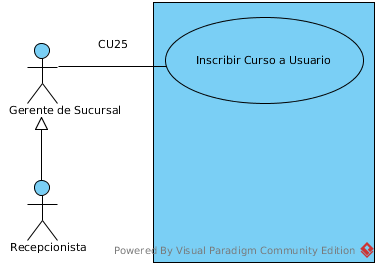
\includegraphics[width=0.4\textwidth]{images/CU25}
  		\caption{CU25 Inscribir a Curso}
		\end{figure}
	}
		\UCitem{Versión}{0.1}
		\UCitem{Actor}{Gerente de Sucursal}
		\UCitem{Propósito}{Que el Gerente de Sucursal pueda llevar acabo el registro de un cliente a todos los cursos solicitados por él.}
		\UCitem{Entradas}{Nombre de Curso,costo horario, fecha de inicio, fecha de termino y numero de Cliente de Gimnasios San Pancho}
		\UCitem{Origen}{Teclado}
		\UCitem{Salidas}{Nombre del curso, Nombre del Instructor, costo, area y horario}
		\UCitem{Destino}{Pantalla}
		\UCitem{Precondiciones}{El Gerente de Sucursal, el curso y el cliente, debe de estar registrado en el sistema. El Gerente de sucursal ya realizo el login para poder tener acceso a todos los privilegios.}
		\UCitem{Postcondiciones}{El cliente quedara asociado a un Curso en el sistema o en su defecto solo consultado en la base de datos .}
		\UCitem{Errores}{Que no se tenga registrado un curso. El curso ya no tiene cúpo}
		\UCitem{Tipo}{Caso de uso primario}
		\UCitem{Observaciones}{Los cursos se pagan cuando el cliente solicita el curso al recepcionista en su sucursal de registro}
		\UCitem{Autor}{Carrillo Mendoza Martín Alejandro.}
		\UCitem{Reviso}{Carrillo Mendoza Martín Alejandro.}
	\end{UseCase}
	\begin{UCtrayectoria}{Principal}
	\UCpaso[\UCactor] Ingresa a la pagina web de \IUref{IU21.0}{Pantalla de Control de Acceso}\label{CU21.0Login} y proporciona su correspondiente nombre de usuario (username) y contraseña (password) para acceder al sistema.
		\UCpaso Válida que el actor se encuentre dado de alta en el sistema. Se utiliza la regla \BRref{BR117}{Determinar si el usuario tiene acceso al sistema.} \Trayref{A}.
		\UCpaso[\UCactor] Al solicitar el registro de un curso a la base de datos,selecciona la pestaña " Alta de Curso  " de la IU21.1 de Menú principal.
		\UCpaso Despliega la \IUref{IU25.1}{Pantalla de Alta de inscribir cliente a un curso} en ella se encuentran los campos: nombre de curso, costo, horario, fecha de inicio,area, fecha de termino,nombre de instructor y su  horario en formato 24:00, todos ellos obligatorios para el registro de un curso en el sistema.
		\UCpaso El sistema carga una nueva pagina  \IUref{IU25.1}{Pantalla de inscribir cliente a un curso} en ella muestra los campos: nombre de curso(varchar), costo(float), fecha de inicio(DATE), fecha de termino(DATE), Numero de Cliente(DATE) y numero de Area(int), todos ellos serán obligatorios y validados para su registro. 
	\UCpaso[\UCactor] Selecciona el nombre del curso a tomar.
	\UCpaso[\UCactor] Selecciona el nombre del instructor a impartir nuevo curso.
	\UCpaso[\UCactor] Selecciona los dias ala semana en los que se imparte nuevo curso.
	\UCpaso[\UCactor] Selecciona el nombre del instructor a impartir nuevo curso.
	\UCpaso[\UCactor] Selecciona la hora en que se impartira un curso (los dias ya seleccionados previamente).
	\UCpaso[\UCactor] Selecciona el area donde se impartira un curso.
	\UCpaso[\UCactor] Confirma el registro de curso a cliente dando click al boton \IUbutton{Enviar} de \label{IU25.1 Inscribir a Curso}.
	\UCpaso Verifica que todos los campos esten llenos ademas con el formato y tipo correspondiente a los datos ubucados en la base de datos. \BRref{BR118}{Validar los datos de un formulario} \Trayref{B}.
		\UCpaso Almacena los datos en la base de datos.
		\UCpaso Muestra el \IUref{UI25.1}{Registro Exitoso de Cliente a curso.}\Trayref{C}.
		\UCpaso Regresa a la pantalla principal de acceso a gerente de sucursal\IUref{IU21.1}{Pantalla de acceso a Gerente de Sucursal}.
\end{UCtrayectoria}

\begin{UCtrayectoriaA}{A}{El actor no introduce nombre de usuario (username) y contraseña (password) para poder ingresar al sistema.}
			\UCpaso Muestra el mensaje {\bf MSG25.0-}``Usuario [{\em y/o}] contraseñas no validos.''.
			\UCpaso[\UCactor] Oprimé el botón \IUbutton{Aceptar}.
			\UCpaso Regresa a la pantalla principal de acceso a gerente de sucursal\IUref{IU21.1}{Pantalla de acceso a Gerente de Sucursal}.
		\end{UCtrayectoriaA}

		\begin{UCtrayectoriaA}{B}{Almenos un campo no esta lleno o no tiene formato adecuado}
			\UCpaso Muestra el mensaje {\bf MSG25.1-}``Uno o más [{\em campos}] no tienen el formato adecuado''.ademas que se tiene obligatoriamente que llenar todos los campos.
			\UCpaso[\UCactor] Oprime el botón \IUbutton{Aceptar}
			\UCpaso[] Termina el caso de uso.
		\end{UCtrayectoriaA}
		
		\begin{UCtrayectoriaA}{C}{Incripcion a curso no fue realizada }
			\UCpaso Muestra el Mensaje {\bf MSG25.2-}El Curso [{\em nombre de curso, costo, horario, fecha de inicio,area, fecha de termino,nombre de instructor y su  horario en formato 24:00 }] no registrado en el sistema, compruebe memoria en el Disco.
			\UCpaso[\UCactor] Oprime el botón \IUbutton{Aceptar}
			\UCpaso[] Termina el caso de uso.
		\end{UCtrayectoriaA}	
%-------------------------------------- TERMINA descripción del caso de uso.